\begin{title}[\Large]
  Параграф 2.4
\end{title}

\begin{title}[\Large]
  Нормальная кривизна кривой. Вторая квадратичная форма поверхности
\end{title}

\begin{define}[нормали к поверхности]
  $\vec \varphi = \vec \varphi(u, \upsilon)$ регулярная поверхность
  $$
  \vec m = \frac{[\vec \varphi_u, \vec \varphi_{\upsilon}]}{|[\vec \varphi_u,
  \vec \varphi_{\upsilon}]|} = \frac{[\vec \varphi_u, \vec \varphi_{\upsilon}]}
  {\sqrt{EG - F^2}} ~ \text{единичная нормаль к поверхности}
  $$
\end{define}

\begin{define}
  $k_n$ проэкция $\stackrel{\bullet \bullet}{\vec \varphi}$ нормального сечения
  на нормаль поверхности называется нормальной кривизной кривой на поверхности.

  $k_g$ проэкция $\stackrel{\bullet \bullet}{\vec \varphi}$ нормального сечения
  на касательную плоскость поверхности называется геодезическая кривизна.

  $k$ кривизна данной кривой на поверхности
  $$
  k^2 = k_g^2 + k_n^2
  $$
  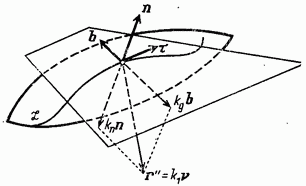
\includegraphics[width = 5cm]{surfaceNormal}
\end{define}

\begin{define}[второй квадратичной формы]
  $$
  \left\{
  \begin{array}{c}
    u = u(s) \\
    \upsilon = \upsilon(s)
  \end{array}
  \right. ~ \text{кривая на поверхности где $s$ натуральный параметр}
  $$
  $\vec \varphi = \vec \varphi(u(s), \upsilon(s))$ уравнение кривой в декартовой
  системе координат

  $k_n = |\stackrel{\bullet \bullet}{\vec \varphi}| \cos \alpha = k \cos \alpha$
  $$
  \stackrel{\bullet}{\vec \varphi} = \vec \varphi_u \stackrel{\bullet}{u} +
  \vec \varphi_{\upsilon} \stackrel{\bullet}{\upsilon}
  $$
  $$
  \stackrel{\bullet \bullet}{\vec \varphi} = \vec \varphi_{uu}
  \stackrel{\bullet}{u^2} + 2\vec \varphi_{u\upsilon}\stackrel{\bullet}{u}
  \stackrel{\bullet}{\upsilon} + \vec \varphi_{\upsilon \upsilon}
  \stackrel{\bullet}{\upsilon^2}
  + \vec \varphi_u \stackrel{\bullet \bullet}{u} +
  \vec \varphi_{\upsilon} \stackrel{\bullet \bullet}{\upsilon}
  $$
  $$
  k_n = (\stackrel{\bullet \bullet}{\vec \varphi}, \vec m) = (\vec \varphi_{uu}
  \stackrel{\bullet}{u^2} + 2\vec \varphi_{u\upsilon}\stackrel{\bullet}{u}
  \stackrel{\bullet}{\upsilon} + \vec \varphi_{\upsilon \upsilon}
  \stackrel{\bullet}{\upsilon^2}
  + \vec \varphi_u \stackrel{\bullet \bullet}{u} +
  \vec \varphi_{\upsilon} \stackrel{\bullet \bullet}{\upsilon}, \vec m) =
  $$
  $$
  = \overbrace{(\vec m, \vec \varphi_{uu})}^L \stackrel{\bullet}{u^2} +
  2\overbrace{(\vec m, \vec \varphi_{u\upsilon})}^M \stackrel{\bullet}{u}
  \stackrel{\bullet}{\upsilon} + \overbrace{(\vec m, \vec \varphi_{\upsilon
  \upsilon})}^N \stackrel{\bullet}{\upsilon^2} =
  $$
  $$
  ds^2 = Ldu^2 + 2Mdud\upsilon + Nd\upsilon^2
  $$
  $$
  = \frac{Ldu^2 + 2Mdud\upsilon + Nd\upsilon^2}{ds^2}
  = \frac{Ldu^2 + 2Mdud\upsilon + Nd\upsilon^2}{Edu^2 + 2Fdu d\upsilon +
  Gd\upsilon^2} = \frac{II}{I}
  $$
  $Ldu^2 + 2M dud\upsilon + Nd\upsilon^2$ вторая квадратичная форма поверхности
\end{define}

\begin{block}[Вычисление нормальной кривизны]
  Нормальная кривизна кривой
  $$
  \left\{
  \begin{array}{c}
    u = u(t) \\
    \upsilon = \upsilon(t)
  \end{array}
  \right. ~~ \text{на регулрной поверхности} ~~ \vec \varphi = \vec \varphi(u,
  \upsilon)
  $$
  вычисляется по формуле
  $$
  k_n = \frac{Lu'^2 + 2Mu'\upsilon' + N\upsilon'^2}{Eu'^2 + 2Fu'\upsilon' +
  G\upsilon'^2}
  $$
  $\Rightarrow$ нормальная кривизна кривой зависит
  только от направления касательных векторов.
\end{block}

\begin{define}[нормального сечения]
  Сечение поверхности плоскостью, содержащей нормаль (в данной точке), образует
  некоторую кривую на поверхности, которая называется нормальным сечением
  поверхности.
\end{define}

\begin{theorem}
  Нормальная кривизна кривой на поверхности равна по абсолютной велечине
  кривезне соответствующего нормального сечения.
\end{theorem}

\begin{proof}
  $k_n = k \cos \alpha$

  $k = k \cos \alpha$

  $1 = \cos \alpha$ $\Rightarrow$ $\alpha = 0$ $\Rightarrow$ $k=k_n$
\end{proof}

\begin{title}[\Large]
  Индикатрисса Дюпена. Главные направления и кривизны
\end{title}

\begin{define}[индикриссы Дюпена]
  Индикрисса Дюпена в точке поверхности $M$ называется кривая в касательной
  плоскости которую описывает конец отрезка длины $\sqrt{R_n}$ начало
  которого находится в точке $M$. $R_n = \frac{1}{k_n}$ радиус нормальной
  кривизны

  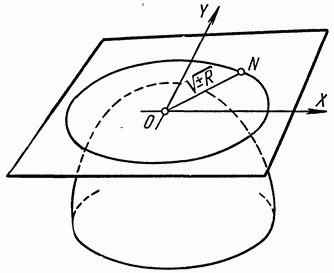
\includegraphics[width = 5cm]{indicatrisaDupena}
\end{define}

\begin{block}[Уравнение индикатрисы Дюпена]
  Выведем уравнение индикатрисы Дюпена. В касательной плоскости выберем аффинную
  систему координа $\vec \varphi_u \vec \varphi_{\upsilon}$ где $P$ лежит на
  индактрисе Дюпена когда $|\overrightarrow{MP}| = \sqrt{R_n}$
  $$
  |\overrightarrow{MP}| = \sqrt{Ex^2 + 2Fxy + Gy^2}
  $$
  $$
  \sqrt{R_n} = \frac{1}{\sqrt{|k_n|}} = \sqrt{\frac{Ex^2 + 2Fxy + Gy^2}{
  |Lx^2 + 2Mxy + Ny^2|}}
  $$
  $$\sqrt{I} = \sqrt{\frac{I}{|II|}}
  $$
  $$
  |Lx^2 + 2Mxy + Ny^2| = 1
  $$
  $$
  Lx^2 + 2Mxy + Ny^2 = \pm 1
  $$
  $$
  \left|
  \begin{array}{cc}
    L & M \\
    M & N
  \end{array}
  \right| = LN - M^2
  $$
  1) $LN - M^2 > 0$ эллипс

  2) $LN - M^2 < 0$ мнимый эллипс $x'^2 - y'^2 = \pm 1$

  3) $LN - M^2 = 0$ пара паралельных прямых $x'^2 = \pm 1$
\end{block}

\begin{define}[главного направления и главной кривизны]
  Направление в касательной плоскости соответствующее направлениям осей симетрии
  индектрисы Дюпена называется главным направлением соответствующие им кривизны
  нормальных сечений называется главными кривизнами и обозначают $k_1, k_2$
\end{define}

\begin{title}[\Large]
  Теорема о приведении пары квадратичных форм поверхности к каноническому виду
\end{title}

\begin{theorem}
  В окрестности каждой точке регулярной кривой поверхности можно выбрать
  параметризацию $(u, \upsilon)$ так что в $M$

  $I(M) = du^2 + d\upsilon^2$

  $II(M) = Ldu^2 + Nd\upsilon^2$ то есть

  $E = |\vec \varphi_u|^2 = 1$

  $F = (\vec \varphi_u, \vec \varphi_{\upsilon}) = 0$

  $G = |\vec \varphi_{\upsilon}|^2 = 1$ в точке $M$

  $\vec \varphi_u, \vec \varphi_{\upsilon}$ ортонормированный базис в
  касательной плоскости в точке $M$

  $Lx^2 + Ny^2 = \pm 1$ уравнение индектрисы Дюпена где оси координат являются
  осями симметрии $\Rightarrow \vec \varphi_u, \vec \varphi_{\upsilon}$ главные
  направления
  $$
  k_n = \frac{II(M)}{I(M)} = \frac{Ldu^2 + Nd\upsilon^2}{du^2 + d\upsilon^2}
  $$
  $$
  \vec \varphi_u = (1,0) ~~~ k_1 = \frac{L 1^2 + N 0^2}{1^2 + 0^2} = L
  $$
  $$
  \vec \varphi_{\upsilon} = (0,1) ~~~ k_2 = N
  $$
  $$
  II(M) = k_1 du^2 + k_2 d\upsilon^2
  $$
\end{theorem}

\begin{title}[\Large]
  Теорема Эйлера о нормальной кривезне кривой и ее следствие
\end{title}

\begin{theorem}[Эйлера]
  $k_n = k_1 \cos^2 \theta + k_2 \sin^2 \theta$ где $\theta$ угол между первым
  главными направлением и направлением нормального сечения.
\end{theorem}

\begin{proof}
  $$
  (du, d\upsilon) = (\cos \theta, \sin \theta)
  $$
  $$
  k_n = \frac{k_1du^2 + k_2d\upsilon^2}{du^2 + d\upsilon^2} = k_1\cos^2 \theta
  + k_2 \sin^2 \theta
  $$
\end{proof}

\begin{block}[Следствие]
  $k_1 \le k_2$ тогда $k_1 \le k_n \le k_2$
\end{block}

\begin{proof}
  $$
  k_n = k_1 \cos^2 \theta + k_2 \sin^2 \theta = k_1 \cos^2 \theta +
  k_1 \sin^2 \theta - k_1 \sin^2 \theta + k_2 \sin^2 \theta =
  $$
  $$
  = k_1 + (k_2 - k_1)\sin^2 \theta ~ \Rightarrow ~ k_1 \le k_n \le k_2 ~~~
  0 \le \sin^2 \theta \le 1
  $$
\end{proof}

\begin{title}[\Large]
  Формулы для вычисления главных направлений и кривизн поверхностей
\end{title}

\begin{theorem}
  Координаты $(du, d\upsilon)$ главных направлений удовлитворяет
  $$
  \left|
  \begin{array}{ccc}
    d\upsilon^2 & -dud\upsilon & d\upsilon^2 \\
    E & F & G \\
    L & M & N
  \end{array}
  \right| = 0
  $$
\end{theorem}

\begin{proof}
  $I = Edu^2 + 2Fdud\upsilon + Gd\upsilon^2$

  $II = Ldu^2 + 2Mdud\upsilon + Ndu^2$

  пусть главные напрвления задаются касательными вектороми
  $\vec a = (\xi_1,\xi_2)$ $\vec b = (\eta_1, \eta_2)$

  1) главные напрвления ортогональны $(\vec a, \vec b) = 0$

  $E\xi_1 \eta_1 + F(\xi_1 \eta_2 + \xi_2 \eta_1) + G\xi_2 \eta_2 = 0$

  $\xi_1(E\eta_1 + F\eta_2) + \xi_2(F\eta_1 + G\eta_2) = 0$

  2) главные направления сопряжены относительно индикатрисы Дюпена

  $$
  \left\{
  \begin{array}{l}
    \xi_1 = -(M\eta_1 + N \eta_2) \\
    \xi_2 = L\eta_1 + M \eta_2
  \end{array}
  \right.
  $$
  $$
  -(M\eta_1 + N\eta_2)(E\eta_1 + F\eta_2) + (L\eta_1 + M\eta_2)(F\eta_1 +
  G\eta_2) = 0
  $$
  $$
  \left|
  \begin{array}{cc}
    E\eta_1 + F\eta_2 & F\eta_1 + G\eta_2 \\
    L\eta_1 + M\eta_2 & M\eta_1 + N\eta_2
  \end{array}
  \right| = 0
  $$
  $$
  \left|
  \begin{array}{cc}
    Edu + Fd\upsilon & Fdu + Gd\upsilon \\
    Ldu + Md\upsilon & Mdu + Nd\upsilon
  \end{array}
  \right| = 0
  $$
  $$
  \left|
  \begin{array}{ccc}
    d\upsilon^2 & -dud\upsilon & d\upsilon^2 \\
    E & F & G \\
    L & M & N
  \end{array}
  \right| = 0
  $$
\end{proof}

\begin{title}[\Large]
  Полная и средняя кривизна поверхности. Классификация точек поверхности
\end{title}

\begin{theorem}
  Главные кривизны поверхности удовлитворяют характеристическому уравнению
  поверхности
  $$
  |II - kI| = 0 ~~~
  \left|
  \begin{array}{cc}
    L - kE & M - kF \\
    M - kF & N - kG
  \end{array}
  \right| = 0
  $$
  $$
  (EG - F^2)k^2 - (LG - 2MF + NE)k + (LN - M^2) = 0
  $$
  $$
  k_1 + k_2 = \frac{LG - 2MF + NE}{EG - F^2}
  $$
  $$
  k_1 k_2 = \frac{LN - M^2}{EG - F^2}
  $$
  $H = \frac{k_1 + k_2}{2}$ среднаяя кривизна поверхности

  $K = k_1 k_2$ полная Гаусова кривизна
  $$
  LN - M^2 > 0
  $$
  $K > 0$ эллипс

  $K < 0$ гиперболическая

  $K = 0$ параболическая
\end{theorem}
